\textbf{Partie A}

\medskip

On considère la fonction $f$ définie sur l'intervalle $[1;+\infty[$ par \[f(x) = \dfrac{\ln x}{x},\] où $\ln$ désigne la fonction logarithme népérien.
%
\begin{enumerate}
	\item Donner la limite de la fonction $f$ en $+\infty$.
	\item On admet que la fonction $f$ est dérivable sur l'intervalle $[1;+\infty[$ et on note $f'$ sa fonction dérivée.
	\begin{enumerate}
		\item Montrer que, pour tout nombre réel $x \geqslant 1$, $f'(x) = \frac{1 - \ln x}{x^2}$.
		\item Justifier le tableau de signes suivant, donnant le signe de $f'(x)$ suivant les valeurs de $x$.
		\begin{center}
			\begin{tikzpicture}
				\tkzTabInit{$x$/0.8,$f'(x)$/0.8}{$1$,$\e$,$+\infty$}
				\tkzTabLine{,+,z,-,}
			\end{tikzpicture}
		\end{center}
		\item Dresser le tableau de variations complet de la fonction $f$.
	\end{enumerate}
	\item Soit $k$ un nombre réel positif ou nul.
	\begin{enumerate}
		\item Montrer que, si $0 \leqslant k \leqslant \dfrac{1}{\text{e}}$, l'équation $f(x) = k$ admet une unique solution sur l'intervalle $[1;\text{e}]$.
		\item Si $k > \dfrac{1}{\text{e}}$, l'équation $f(x) = k$ admet-elle des solutions sur l'intervalle $[1;+\infty[$ ?
		
		Justifier.
	\end{enumerate}
\end{enumerate}

\textbf{Partie B}

\medskip

Soit $g$ la fonction définie sur $\R$ par : \[g(x) = \text{e}^{\frac{x}{4}}.\]
%
On considère la suite $\left(u_n\right)$ définie par $u_0 = 1$ et, pour tout entier naturel $n$ :

\hfill$u_{n+1} = \text{e}^{\frac{u_n}{4}}$ c'est-à-dire : $u_{n+1} = g\left(u_n\right)$.\hfill~
%
\begin{enumerate}
	\item Justifier que la fonction $g$ est croissante sur $\R$.
	\item Montrer par récurrence que, pour tout entier naturel $n$, on a : $u_n \leqslant  u_{n+1} \leqslant \text{e}$.
	\item En déduire que la suite $\left(u_n\right)$ est convergente.
\end{enumerate}

On note $\ell$ la limite de la suite $\left(u_n\right)$ et on admet que $f$ est solution de l'équation : \[\text{e}^{\frac{x}{4}} = x.\]
%
\begin{enumerate}[resume]
	\item En déduire que $\ell$ est solution de l'équation $f(x) = \dfrac14$, où $f$ est la fonction étudiée dans
	la \textbf{partie A}.
	\item Donner une valeur approchée à $10^{-2}$ près de la limite $\ell$ de la suite $\left(u_n\right)$.
\end{enumerate}

